\documentclass[12pt, twoside]{article}
\usepackage[letterpaper, margin=1in, headsep=0.2in]{geometry}
\setlength{\headheight}{0.6in}
%\usepackage[english]{babel}
\usepackage[utf8]{inputenc}
\usepackage{microtype}
\usepackage{amsmath}
\usepackage{amssymb}
%\usepackage{amsfonts}
\usepackage{siunitx} %units in math. eg 20\milli\meter
\usepackage{yhmath} % for arcs, overparenth command
\usepackage{tikz} %graphics
\usetikzlibrary{quotes, angles}
\usepackage{graphicx} %consider setting \graphicspath{{images/}}
\usepackage{parskip} %no paragraph indent
\usepackage{enumitem}
\usepackage{multicol}
\usepackage{venndiagram}

\usepackage{fancyhdr}
\pagestyle{fancy}
\fancyhf{}
\renewcommand{\headrulewidth}{0pt} % disable the underline of the header
\raggedbottom
\hfuzz=2mm %suppresses overfull box warnings

\usepackage{hyperref}

\fancyhead[LE]{\thepage}
\fancyhead[RO]{\thepage \\ Name: \hspace{4cm} \,\\}
\fancyhead[LO]{BECA / Dr. Huson / Geometry\\*  Unit 10: Similarity and proportions \\* 20 March 2023}

\begin{document}

\subsubsection*{10.1 Homework: Mixed review}
\begin{enumerate}
  \item In  $\triangle ABC$ shown below, $m\angle A=(3x+4)^\circ$, $m\angle B=(5x-15)^\circ$, and $m\angle C=(x-7)^\circ$. What is $m\angle A$?\\[0.5cm]
  \begin{tikzpicture}
    \draw [thick]
      (2,0)node[below]{$A$}--
      (9,0)node[below]{$C$}--
      (4,3)node[above]{$B$} --(2,0);
      \node at (3.3,0)[above]{$(3x+4)^\circ$};
      \node at (8.2,0)[above left]{$(x-7)^\circ$};
      \node at (4.4,2.3)[below]{$(5x-15)^\circ$};
  \end{tikzpicture} \vspace{4cm}

\item Given two parallel lines and a transversal, as shown below.
  \begin{center}
  \begin{tikzpicture}
    \draw [<->, thick] (1,2)--(9,2);
    \draw [<->, thick] (0,0)--(8,0);
    \draw [<->, thick] (4,-1)--(5.5,3);
    \node at (4.5,0.3) [left]{$5$};
    \node at (4.5,0.3) [right]{$6$};
    \node at (4.3,-0.3) [left]{$7$};
    \node at (4.3,-0.3) [right]{$8$};
    \node at (5.2,2) [above left]{$1$};
    \node at (5.2,2) [above right]{$2$};
    \node at (5,2) [below left]{$3$};
    \node at (5,2) [below right]{$4$};
  \end{tikzpicture}
  \end{center}
  \begin{enumerate}
    \item State the angle corresponding with $\angle 5$. \vspace{1cm}
    \item Given $m\angle 3 = 78^\circ$ and $m\angle 5 = 3x^\circ$. Find $x$. \vspace{3.5cm}
    \item In a proof, what reason would justify $\angle 3 \cong \angle 6$? \rule{6cm}{0.15mm}
  \end{enumerate}

\item Given two parallel lines and a transversal, as shown. Apply the theorem, ``If a transversal intersects two parallel lines, then corresponding angles are congruent."
  \begin{center}
  \begin{tikzpicture}
    \draw [<->, thick] (1,2)--(9,2);
    \draw [<->, thick] (0,0)--(8,0);
    \draw [<->, thick] (4,-1)--(5.5,3);
    \node at (4.5,0.3) [left]{$5$};
    \node at (4.5,0.3) [right]{$6$};
    \node at (4.3,-0.3) [left]{$7$};
    \node at (4.3,-0.3) [right]{$8$};
    \node at (5.2,2) [above left]{$1$};
    \node at (5.2,2) [above right]{$2$};
    \node at (5,2) [below left]{$3$};
    \node at (5,2) [below right]{$4$};
  \end{tikzpicture}
  \end{center}
  \begin{enumerate}
    \item State the angle corresponding with $\angle 2$. \vspace{1cm}
    \item Given $m\angle 4 = 115^\circ$ and $m\angle 6 = 5x^\circ$. Find $x$. \vspace{3cm}
    \item Given $m\angle 7 = 65^\circ$. Find $m\angle 2$. \vspace{2cm}
    \item In a proof, what reason would justify $\angle 4 \cong \angle 5$? \rule{6cm}{0.15mm}
  \end{enumerate}

\item The image of triangle $ABC$ after a translation is $\triangle A'B'C'$. Is the area of the triangle greater, smaller, or the same after the translation? Justify your answer.

\newpage  
\item Given $m\angle K=38^\circ$ and $m\angle KNL=111^\circ$. Find $m\angle M$.\\[1cm]
 \begin{tikzpicture}
   %\draw [->, thick] (0,0)--(5,5);
   \draw [<-, thick] (8,0)--(0,0)--(3,3)--(4.5,0);
   \draw [fill] (0,0) circle [radius=0.05] node[below]{$M$};
   \draw [fill] (4.5,0) circle [radius=0.05] node[below]{$N$};
   \draw [fill] (3,3) circle [radius=0.05] node[right]{$K$};
   \draw [fill] (7,0) circle [radius=0.05] node[below]{$L$};
 \end{tikzpicture}
 \vspace{3cm}

\item Given $m\angle R=53^\circ$ and $m\angle UST=117^\circ$. Find $m\angle U$.\\[1cm]
  \begin{tikzpicture}
    %\draw [->, thick] (0,0)--(5,5);
    \draw [<-, thick] (8,0)--(0,0)--(3,3)--(4.5,0);
    \draw [fill] (0,0) circle [radius=0.05] node[below]{$R$};
    \draw [fill] (4.5,0) circle [radius=0.05] node[below]{$S$};
    \draw [fill] (3,3) circle [radius=0.05] node[right]{$U$};
    \draw [fill] (7,0) circle [radius=0.05] node[below]{$T$};
  \end{tikzpicture}
  \vspace{3cm}

\item In  $\triangle ABC$ shown below, side $\overline{AC}$ is extended to point $D$ with $m\angle DAB=(180-2x)^\circ$, $m\angle C=(x-10)^\circ$, and $m\angle B=(3x+10)^\circ$.
  \begin{center}
    \begin{tikzpicture}
      \draw [thick](-1.5,0)node[below]{$D$}--
        (1.8,0)node[below]{$A$}--
        (9,0)node[below]{$C$}--
        (4,3)node[above]{$B$} --(2,0);
        \node at (2.2,0)[above left]{$(180-2x)^\circ$};
        \node at (8.2,0)[above left]{$(x-10)^\circ$};
        \node at (4.4,2.4)[below]{$(3x+10)^\circ$};
    \end{tikzpicture}
  \end{center}
  What is $m\angle BAC$?

\newpage
\item On the graph below, draw $\overline{AB}$, with $A(-2,1)$ and $B(6,3)$, labeling the end points. Determine and state the coordinates of the midpoint $M$ of $\overline{AB}$ and mark and label it on the graph.\\
\begin{tikzpicture}[scale=.635]
  \draw [help lines] (-3,-2) grid (8,6);
  \draw [thick, ->] (-3.2,0) -- (8.4,0) node [below right] {$x$};
  \draw [thick, ->] (0,-2.2)--(0,6.4) node [left] {$y$};
\end{tikzpicture}
\vspace{2cm}

\item On the graph below, draw $\overline{AB}$, with $A(-1,5)$ and $B(7,0)$, labeling the end points. Determine and state the coordinates of the midpoint $M$ of $\overline{AB}$ and mark and label it on the graph.\\
    \begin{tikzpicture}[scale=.635]
      \draw [help lines] (-3,-2) grid (8,7);
      \draw [thick, ->] (-3.2,0) -- (8.4,0) node [below right] {$x$};
      \draw [thick, ->] (0,-2.2)--(0,7.4) node [left] {$y$};
    \end{tikzpicture}
    \vspace{1cm}

\item In the diagram below, $\overleftrightarrow{AC}$ has endpoints with coordinates $A(-3,2)$ and $C(3, -7)$.
  \begin{center} %4 quadrant regents grid
    \begin{tikzpicture}[scale=.48]
      \draw [help lines] (-8,-9) grid (8,5);
      \draw [thick, <->] (-8.2,0) -- (8.4,0) node [below right] {$x$};
      \draw [thick, <->] (0,-9.2)--(0,5.4) node [left] {$y$};
      \draw [thick] (-3,2)--(3,-7);
      \draw [fill] (-3,2) circle [radius=0.1] node[above left] {$A$};
      \draw [fill] (3,-7) circle [radius=0.1] node[below right] {$C$};
    \end{tikzpicture}
  \end{center}
  If $B$ is a point on  and $AB {:} BC = 1{:}2$,  what  are  the  coordinates of $B$?

\newpage
\item Apply the translation $(x,y) \rightarrow (x-1,y+3)$ to the point $A(0,-4)$. \vspace{1cm}

\item Apply the translation $(x,y) \rightarrow (x+1,y+6)$ to the point $A(-5,3)$. \vspace{2cm}

\item What is the image of $B(2,5)$ under a reflection across the $y$-axis? \vspace{2cm}

\item State the translation that would map $C(2,-3)$ onto $C'(5,-4)$. \vspace{1cm}

\item What is the image of $B(4,3)$ under a reflection across the $x$-axis? \vspace{1cm}

\item State the translation that would map $C(1,5)$ onto $C'(4,3)$. \vspace{1cm}

\item Express the result to the nearest thousandth.  \vspace{0.5cm}
  \begin{multicols}{2}
    \begin{enumerate}
      \item $\sin 30^\circ = $ \vspace{0.5cm}
      \item $\tan 45^\circ =$
      \item $\sin 28^\circ = $ \vspace{0.5cm}
      \item $\cos 25^\circ =$
    \end{enumerate}
  \end{multicols}

\item Express the result to \emph{the nearest thousandth}.  \vspace{0.5cm}
  \begin{multicols}{2}
    \begin{enumerate}
      \item $\sin 60^\circ = $ \vspace{0.5cm}
      \item $\cos 23^\circ =$
      \item $\tan 45^\circ = $ \vspace{0.5cm}
      \item $\sin 81^\circ =$
    \end{enumerate}
  \end{multicols}

\item Express the result to the nearest thousandth.  %\vspace{0.5cm}
\begin{multicols}{2}
  \begin{enumerate}
    \item $\cos 60^\circ = $ \vspace{0.5cm}
    \item $\tan 45^\circ =$
    \item $\sin 48^\circ = $ \vspace{0.5cm}
    \item $\cos 15^\circ =$
  \end{enumerate}
\end{multicols}

\item Express the result to the nearest thousandth.  \vspace{1cm}
  \begin{multicols}{2}
    \begin{enumerate}
      \item $\cos 60^\circ = $ \vspace{1cm}
      \item $\tan 25^\circ =$
      \item $\sin 41^\circ = $ \vspace{1cm}
      \item $\cos 75^\circ =$
    \end{enumerate}
  \end{multicols} \vspace{1cm}

\item Find the image of $A(3,2)$ after a translation four to the right and down two. \vspace{1cm}

\item Apply the translation $(x,y) \rightarrow (x-5,y+1)$ to the point $B(-2,-1)$. \vspace{1cm}

\item State the translation that would map $C(6,3)$ onto $C'(5,13)$.
  
\item $\triangle ABC$ is shown with $m\angle C=90^\circ$. The lengths of the triangle's sides are $a$, $b$, and $c$.
  \begin{center}
    \begin{tikzpicture}[scale=0.7]
      \draw [thick]
      (0,0)node[left]{$A$}--
      (4,0)node[below right]{$C$}--
      (4,5)node[right]{$B$}--cycle;
      \node at (2,0)[below]{$b$};
      \node at (4,2.7)[right]{$a$};
      \node at (1.8,2.5)[above]{$c$};
    \end{tikzpicture} %\vspace{1cm}
  \end{center}
  Express each trigonometric ratio as a fraction of two variables.
  \begin{multicols}{2}
    \begin{enumerate}
    \item $\sin A =$ \vspace{0.5cm}
    \item $\cos A =$ \vspace{0.5cm}
    \item $\tan A =$
    \item $\sin B =$ \vspace{0.5cm}
    \item $\cos B =$ \vspace{0.5cm}
    \item $\tan B =$
  \end{enumerate}
\end{multicols}

\item Given right $\triangle ABC$ with $AC=12, BC=5, AB=13$, $m\angle C=90^\circ$. Express each trig ratio as a fraction.
    \begin{center}
      \begin{tikzpicture}[scale=1]
        \draw [thick](0,0)--(6,0)--(6,2.5)--(0,0);
        \draw [fill] (0,0) circle [radius=0.05] node[below]{$A$};
        \draw [fill] (6,0) circle [radius=0.05] node[below]{$C$};
        \draw [fill] (6,2.5) circle [radius=0.05] node[above right]{$B$};
      \end{tikzpicture} \vspace{1cm}
    \end{center}
    \begin{multicols}{2}
      \begin{enumerate}
        \item $\sin A = $ \vspace{1cm}
        \item $\cos A =$
        \item $\sin B = $ \vspace{1cm}
        \item $\tan B =$
      \end{enumerate}
    \end{multicols}

\item Given right $\triangle ABC$ with $m\angle C=90^\circ$, $m\angle A = 30^\circ$, and $AB=12$.
  \begin{center}
    \begin{tikzpicture}%[scale=0.7]
      \draw [thick](0,0)--(6,0)--(6,3)--(0,0);
      \draw [fill] (0,0) circle [radius=0.05] node[below]{$A$};
      \draw [fill] (6,0) circle [radius=0.05] node[below]{$C$};
      \draw [fill] (6,3) circle [radius=0.05] node[above right]{$B$};
    \end{tikzpicture} %\vspace{2cm}
  \end{center}
  \begin{enumerate}
    \item Find $AC$. \vspace{3cm}
    \item Find $BC$. \vspace{3cm}
  \end{enumerate}

\item Given right $\triangle JKL$ with $\overline{JK} \perp \overline{KL}$, $JL=11$, $m\angle J=29^\circ$.
  \begin{center}
    \begin{tikzpicture}[scale=0.7]
      \draw [thick](0,0)--(7,0)--(7,3)--(0,0);
      \draw [fill] (0,0) circle [radius=0.05] node[below]{$J$};
      \draw [fill] (7,0) circle [radius=0.05] node[below]{$K$};
      \draw [fill] (7,3) circle [radius=0.05] node[above right]{$L$};
    \end{tikzpicture}
  \end{center}
  \begin{enumerate}
    \item Find the length $JK$ \vspace{1.25cm}
    \item Find the length $KL$
  \end{enumerate}
  
\item $\triangle ABC$ is shown with $m\angle C=90^\circ$. The lengths of the triangle's sides are $a$, $b$, and $c$. Express each trigonometric ratio as a fraction of two variables. \vspace{1cm}
  \begin{multicols}{2}
    \begin{tikzpicture}[scale=0.7]
      \draw [thick]
      (0,0)node[left]{$A$}--
      (4,0)node[below right]{$C$}--
      (4,5)node[right]{$B$}--cycle;
      \node at (2,0)[below]{$b$};
      \node at (4,2.7)[right]{$a$};
      \node at (1.8,2.5)[above]{$c$};
    \end{tikzpicture}

    \begin{enumerate}
    \item $\sin A =$ \vspace{0.75cm}
    \item $\cos A =$ \vspace{0.75cm}
    \item $\tan A =$
  \end{enumerate}
\end{multicols}

\newpage
\item Using  a  compass  and  straightedge,  construct  the  median  to  side $\overline{BC}$ in $\triangle ABC$ below.\\ (Leave all construction marks.)
  \vspace{1cm}
  \begin{center}
  \begin{tikzpicture}
  \draw [<->, thick]
    (0,0) node[left]{$A$}--
    (10,-2) node[right]{$B$}--
    (4,-5) node[below]{$C$}
    --cycle;
  \end{tikzpicture}
  \end{center} \vspace{2cm}

\item With a compass and straightedge, construct a square inscribed in circle $P$. (Leave all construction marks.)
\vspace{1cm}
\begin{center}
\begin{tikzpicture}
\draw [thick] (0,0) circle [radius=4cm];
\draw [fill] (0,0) circle [radius=0.05] node[below]{$P$};
\end{tikzpicture}
\end{center}

\newpage
\item $A(3,1)$ is one endpoint of $\overline{AB}$. The segment's midpoint is $M(7,6)$. Find the other endpoint, $B$. \vspace{5cm}

\item $M(5,5)$ is the midpoint of $AB$. Given $A(2,3)$, find the other endpoint, $B$. \vspace{2cm}

\item The line $l$ has the equation $y=\frac{1}{2} x-3$.
  \begin{enumerate}
    \item What is the slope of the line $k$, given $k \parallel l$?
    \vspace{1cm}
    \item What is the slope of the line $m$, given $m \perp l$?
    \vspace{1cm}
  \end{enumerate}

\item The line $l$ has the equation $y=-\frac{3}{2} x-7$.
  \begin{enumerate}
    \item What is the slope of the line $k$, given $k \parallel l$?
    \vspace{1.5cm}
    \item What is the slope of the line $m$, given $m \perp l$?
    \vspace{2.5cm}
  \end{enumerate}

\item Given $P(-2,9)$ and $Q(3,-3)$, find the length of $\overline{PQ}$.
  \vspace{4cm}

\item A translation maps $A(5,2) \rightarrow A'(-2,3)$. What is the image of $B(-1,5)$ under the same translation?  \vspace{0.5cm}

\newpage
\item Apply the translation $(x,y) \rightarrow (x-2,y+4)$ to the point $A(2,-1)$. \vspace{2cm}
\item What is the image of $B(2,7)$ under a reflection across the $x$-axis? \vspace{2cm}
\item State the translation that would map $C(-3,1)$ onto $C'(4,0)$. \vspace{3cm}
\item A translation maps $D(1,9) \rightarrow D'(4,3)$. What is the image of $E(6,-2)$ under the same translation?  \vspace{3cm}

\item The image of triangle $ABC$ after a translation is $\triangle A'B'C'$. Is the area of the triangle greater, smaller, or the same after the translation? Justify your answer.

\newpage
\item In  $\triangle ABC$ shown below, side $\overline{AC}$ is extended to point $D$ with $m\angle DAB=(180-4x)^\circ$, $m\angle C=(x+2)^\circ$, and $m\angle B=(6x-9)^\circ$. \\[1cm]
  \begin{center}
    \begin{tikzpicture}
      \draw [thick](-1.5,0)node[below]{$D$}--
        (1.8,0)node[below]{$A$}--
        (9,0)node[below]{$C$}--
        (4,3)node[above]{$B$} --(2,0);
        \node at (2.2,0)[above left]{$(180-4x)^\circ$};
        \node at (8.2,0)[above left]{$(x+2)^\circ$};
        \node at (4.4,2.4)[below]{$(6x-9)^\circ$};
    \end{tikzpicture}
  \end{center} \vspace{0.5cm}
  What is $m\angle BAC$?

\newpage
\item Given right $\triangle JKL$ with $\overline{JK} \perp \overline{KL}$, $JL=9$, $m\angle J=32^\circ$. Find the length $JK$, \emph{rounded to the nearest thousandth}.
  \begin{center}
  \begin{tikzpicture}[scale=0.7]
    \draw [thick]
    (0,0) node[below]{$J$}--
    (7,0)  node[below]{$K$}--
    (7,3) node[above right]{$L$}--cycle;
  \end{tikzpicture}
  \end{center} \vspace{4cm}

\item Spicy: In the diagram below, $\overleftrightarrow{AC}$ has endpoints with coordinates $A(-2,3)$ and $C(8, -2)$.
  \begin{center} %4 quadrant regents grid
    \begin{tikzpicture}[scale=.48]
      \draw [help lines] (-7,-5) grid (9,7);
      \draw [thick, <->] (-7.4,0) -- (9.4,0) node [below right] {$x$};
      \draw [thick, <->] (0,-5.4)--(0,7.4) node [left] {$y$};
      \draw [thick] (-2,3)--(8, -2);
      \draw [fill] (-2,3) circle [radius=0.1] node[above left] {$A$};
      \draw [fill] (8, -2) circle [radius=0.1] node[below right] {$C$};
    \end{tikzpicture}
  \end{center}
  If $B$ is a point on $\overline{AC}$ and $AB {:} BC = 2{:}3$,  what  are  the  coordinates of $B$?

\newpage
\item Spicy: Triangle $\triangle TEN$ is graphed on the set of axes below. The vertices of $\triangle TEN$ have the coordinates $T(-1,-2)$, $E(8,1)$, and $N(3,6)$.
  \begin{center} %4 quadrant regents grid
  \begin{tikzpicture}[scale=.48]
  \draw [help lines] (-8,-5) grid (10,9);
  \draw [thick, <->] (-8.4,0) -- (10.4,0) node [below right] {$x$};
  \draw [thick, <->] (0,-5.4)--(0,9.4) node [left] {$y$};
  \draw [thick] (-1,-2) node[below] {$T$}--
  (8,1) node[right] {$E$}--
  (3,6) node[above] {$N$}--
  cycle;
  %\draw [fill] (5,0) circle [radius=0.1] node[above left] {$P$};
  \end{tikzpicture}
  \end{center}
  \begin{enumerate}
  \item Draw an altitude through point $N$ perpendicular to $\overline{TE}$.
  \item What is the length of the altitude drawn through $N$? \vspace{3.5cm}
  \item What is the length of the base, $TE$?  \vspace{3.5cm}
  \item Find the area of  $\triangle DAN$.
  \end{enumerate}




\end{enumerate}
\end{document}
